\chapter{Arhitektura i dizajn sustava}
		
		{Arhitekturu možemo podijeliti na 3 podsustava:}

		\begin{packed_item}
			\item {Korisničko sučelje (frontend)}
			\item {Poslužitelj (backend)}
			\item {Baza podataka}\vspace{0.1cm}
		\end{packed_item}

		{\underbar{Web preglednik} (\textit{Internetski preglednik, Web browser, Internet browser})  je program koji korisniku omogućuje pregled web-stranica i multimedijalnih sadržaja vezanih uz njih. Svaki internetski preglednik je \underbar{interpreter} (program koji u realnom vremenu izvršava izvorni kod napisan u nekom programskom jeziku, umjesto da ga, prije izvršavanja cijelog prevede u strojni jezik, što inače radi jezični prevoditelj). Dakle, stranica je pisana u kodu koji preglednik interpretira u čitljiv sadržaj. Korisnici putem web preglednika šalju zahtjeve poslužitelju.}\vspace{0.3cm}

		{\underbar{Web poslužitelj} je temelj svake Web aplikacije jer on služi za komunikaciju klijenta s aplikacijom. Takva vrsta komunikacije odvija se uz pomoć HTTP (\textit{Hyper Text Transfer Protocol}) protokola koji predstavlja glavnu i najčešću metodu prijenosa informacija na Webu. Osnovna namjena ovog protokola je omogućavanje objavljivanja i prezentacije HTML dokumenata, tj. Web stranica. Poslužitelj nam dakle služi za prosljeđivanje zahtjeva Web aplikaciji te je zadužen za njezino pokretanje.}\vspace{0.3cm}

		{Od ostalih protokola koji služe za komunikaciju i prijenos informacija i podataka između klijenta i poslužitelja treba napomenuti: IP (\textit{Internet Protocol}) koji služi za prijenos podataka u blokovima (paketi, datagrami), komunikacijski protokol ARP (\textit{Address Resolution Protocol}) te ICMP (\textit{Internet Control Message Protocol}) koji je ugrađen u svaki IP modul kako bi omogućio računalima slanje kontrolnih poruka o greškama. ICMP prijavljuje greške, ali nije zadužen za njihovo ispravljanje.}\vspace{0.3cm}

		{Klijent koristi korisničko sučelje, tj. Web aplikaciju, prikazanu u pregledniku, te preko nje šalje zahtjeve poslužitelju. Nakon obrade podataka, poslužitelj vraća odgovor aplikaciji koja ga potom prikazuje korisniku.}\vspace{0.3cm}
		
		\begin{figure}[H]
		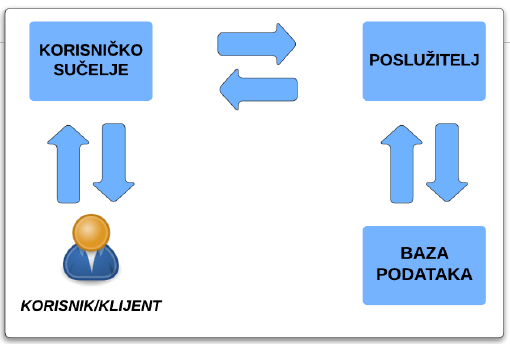
\includegraphics[scale=1]{slike/ArhitekturaSustava.png}
		\centering
		\caption{Prikaz arhitekture sustava}
		\label{fig:ArhitekturaSustava}
		\end{figure}

		{Programski i korisnički jezici koje smo koristili su: HTML, CSS i JavaScript za Frontend te Java za Backend. Radni okviri koje smo odabrali su React (Frontend) i Spring Boot (Backend). Od razvojnih okruženja koristili smo IntelliJ u okviru izrade Backenda te Visual Studio Code za izradu Frontenda.}\vspace{0.3cm}

		{U okviru Backenda korišten je REST (\textit{Representational State Transfer}) API (\textit{Application programming Interface}). \underbar{REST} je softverska arhitektura koja nameće uvjete o tome kako API treba raditi, a \underbar{API} definira pravila koja morate slijediti za komunikaciju s drugim softverskim sustavima.}\vspace{0.3cm}

		{\underbar{REST API} je sučelje koje dva računalna sustava koriste za sigurnu razmjenu informacija putem interneta. Većina Web aplikacija mora komunicirati s drugim internim aplikacijama i aplikacijama trećih strana kako bi izvršile razne zadatke, a REST API podržava ovu razmjenu informacija jer slijedi sigurne, pouzdane i učinkovite softverske komunikacijske standarde.}\pagebreak
		
		
		\section{Baza podataka}
		
%		\textit{Dio 1. implementacije}
			
		{Podaci u aplikaciji će se spremati u relacijsku bazu podataka koristeći Postgres kao DBMS. Baza će se sastojati od sljedećih entiteta:}
		\begin{itemize}
			\item Korisnik
			\item Mjesto
			\item Tvrtka
			\item Zaposlenik
			\item Projekt
			\item ProjectFRTeamMembers
			\item Suradnja
		\end{itemize}
			\subsection{Opis tablica}

				\begin{longtblr}[
					label=none,
					entry=none
					]{
						width = \textwidth,
						colspec={|X[14,l]|X[10, l]|X[20, l]|}, 
						rowhead = 1,
					} %definicija širine tablice, širine stupaca, poravnanje i broja redaka naslova tablice
						\hline \multicolumn{3}{|c|}{\textbf{Korisnik}}	 \\ \hline[3pt]
						\SetCell{LightGreen}IDKorisnik & INT & ID korisnika  	\\ \hline
						Ime	& VARCHAR(40) & Ime korisnika \\ \hline 
						Prezime & VARCHAR(40) & Prezime korisnika \\ \hline 
						Nadimak & VARCHAR(40) & Nadimak korisnika \\ \hline 
        				LoginEmail & VARCHAR(60) & Email adresa pomoću kojeg se korisnik logira \\ \hline 
        				NotificationEmail & VARCHAR(60) & Email adresa na koju korisnik prima obavijesti \\ \hline 
						MaxRazinaOvlasti & INT & Maksimalna razina ovlasti koju korisnik posjeduje (ENUM) \\ \hline
        				Opis & VARCHAR(480) & Opis korisnika \\ \hline 
				\end{longtblr}

				\begin{longtblr}[
					label=none,
					entry=none
					]{
						width = \textwidth,
						colspec={|X[14,l]|X[10, l]|X[20, l]|}, 
						rowhead = 1,
					} %definicija širine tablice, širine stupaca, poravnanje i broja redaka naslova tablice
					\hline \multicolumn{3}{|c|}{\textbf{Mjesto}}	 \\ \hline[3pt]
					\SetCell{LightGreen} PBr & INT & Poštanski broj mjesta \\ \hline
					Naziv & VARCHAR(120) & Naziv mjesta \\ \hline
				\end{longtblr}

				\begin{longtblr}[
					label=none,
					entry=none
					]{
						width = \textwidth,
						colspec={|X[14,l]|X[10, l]|X[20, l]|}, 
						rowhead = 1,
					} %definicija širine tablice, širine stupaca, poravnanje i broja redaka naslova tablice
						\hline \multicolumn{3}{|c|}{\textbf{Tvrtka}}	 \\ \hline[3pt]
						\SetCell{LightGreen} IDTvrtka & INT	&  Id tvrtke	\\ \hline
						Naziv & VARCHAR(60) & Naziv tvrtke \\ \hline 
						Podrucje & VARCHAR(40) &  Područje kojim se tvrtka bavi \\ \hline 
						ABCKategorizacija & CHAR & Kategorija tvrtke (ENUM: A, B ili C) \\ \hline 
                        MjesecPlaniranjaBudzeta & INT & Mjesec u kojem tvrtka planira budžet \\ \hline
                        Drzava & VARCHAR(60) & Država u kojoj tvrtka posluje \\ \hline
                        \SetCell{LightBlue} PBr & INT & Poštanski broj mjesta tvrtke \\ \hline
                        Adresa & VARCHAR(120) & Adresa tvrtke \\ \hline
                        WebURL & VARCHAR(60) & Adresa web stranice tvrtke \\ \hline
                        Kontaktirati & BOOLEAN & Treba li ubuduće tu tvrtku kontaktirati \\ \hline
				\end{longtblr}

				\begin{longtblr}[
					label=none,
					entry=none
					]{
						width = \textwidth,
						colspec={|X[14,l]|X[10, l]|X[20, l]|}, 
						rowhead = 1,
					} %definicija širine tablice, širine stupaca, poravnanje i broja redaka naslova tablice
					\hline \multicolumn{3}{|c|}{\textbf{Zaposlenik}}	 \\ \hline[3pt]
						\SetCell{LightGreen} IDZaposlenik & INT	& Id zaposlenika \\ \hline
						\SetCell{LightBlue} IDTvrtka & INT & Id tvrtke za koju zaposlenik radi\\ \hline 
						Ime & VARCHAR(40) & Ime zaposlenika \\ \hline 
						Prezime & VARCHAR(40) & Prezime zaposlenika \\ \hline
						Email & VARCHAR(60)	& Email adresa zaposlenika \\ \hline
						Tel & VARCHAR(20) & Broj telefona zaposlenika \\ \hline
						Uloga & VARCHAR(40)	& Pozicija zaposlenika u tvrtki (npr. PR) \\ \hline
						Opis & VARCHAR(60) & Opis zaposlenika (npr. glavni kontakt) \\ \hline 
				\end{longtblr}

				\begin{longtblr}[
					label=none,
					entry=none
					]{
						width = \textwidth,
						colspec={|X[14,l]|X[10, l]|X[20, l]|}, 
						rowhead = 1,
					} %definicija širine tablice, širine stupaca, poravnanje i broja redaka naslova tablice
					\hline \multicolumn{3}{|c|}{\textbf{Projekt}}	 \\ \hline[3pt]
					\SetCell{LightGreen}IDProjekt & INT	& ID projekta \\ \hline
					Naziv & VARCHAR(40) & Naziv projekta \\ \hline 
					Kategorija & INT & Kategorija u koju spada projekt \\ \hline 
					Tip & INT & Tip projekta (ENUM: eksterni ili interni) \\ \hline 
					ProjektPocetak & TIMESTAMP & Datum početka projekta \\ \hline 
					ProjektZavrsetak & TIMESTAMP & Datum završetka projekta \\ \hline
					\SetCell{LightBlue} IDFRResp & INT & ID korisnika odgovornog za odnose s tvrtkama projekta \\ \hline
					FRCilj & INT & Količina novca koja se želi prikupiti za projekt \\ \hline
					PrviFRPing & TIMESTAMP & Datum prvog "ping"-a \\ \hline
					DrugiFRPing & TIMESTAMP & Datum drugog "ping"-a \\ \hline
				\end{longtblr}

				\begin{longtblr}[
					label=none,
					entry=none
					]{
						width = \textwidth,
						colspec={|X[14,l]|X[10, l]|X[20, l]|}, 
						rowhead = 1,
					} %definicija širine tablice, širine stupaca, poravnanje i broja redaka naslova tablice
					\hline \multicolumn{3}{|c|}{\textbf{ProjectFRMembers}}	 \\ \hline[3pt]
					\SetCell{LightGreen}IDKorisnik & INT & Id korisnika koji je FR team member projekta \\ \hline
					\SetCell{LightGreen}IDProjekt & INT & Id projekta \\ \hline
				\end{longtblr}

				\begin{longtblr}[
					label=none,
					entry=none
					]{
						width = \textwidth,
						colspec={|X[14,l]|X[10, l]|X[20, l]|}, 
						rowhead = 1,
					} %definicija širine tablice, širine stupaca, poravnanje i broja redaka naslova tablice
					\hline \multicolumn{3}{|c|}{\textbf{Suradnja}}	 \\ \hline[3pt]
					\SetCell{LightGreen}IDProjekt & INT	& Id projekta \\ \hline
			                \SetCell{LightGreen}IDTvrtka & INT	& Id tvrtke \\ \hline
					\SetCell{LightBlue}IDOdgovoran & INT & Id korisnika odgovornog za suradnju s tvrtkom \\ \hline 
					\SetCell{LightBlue}IDKontakt & INT & Id kontakt osobe u tvrtci \\ \hline 
					Kategorija & VARCHAR(20) & Kategorija suradnje (ENUM: financijska, materijalna ili akademska) \\ \hline
					Status & VARCHAR(20) & Kontaktirano, ping, dopis, sastanak, uspješno ili neuspješno \\ \hline
					Komentar & VARCHAR(480) & Komentar na suradnju \\ \hline
					Vrijednost & INT & Ostvarena novčana vrijednost suradnje \\ \hline
				\end{longtblr}
				
			
			\subsection{Dijagram baze podataka}
				\begin{figure}[H]
					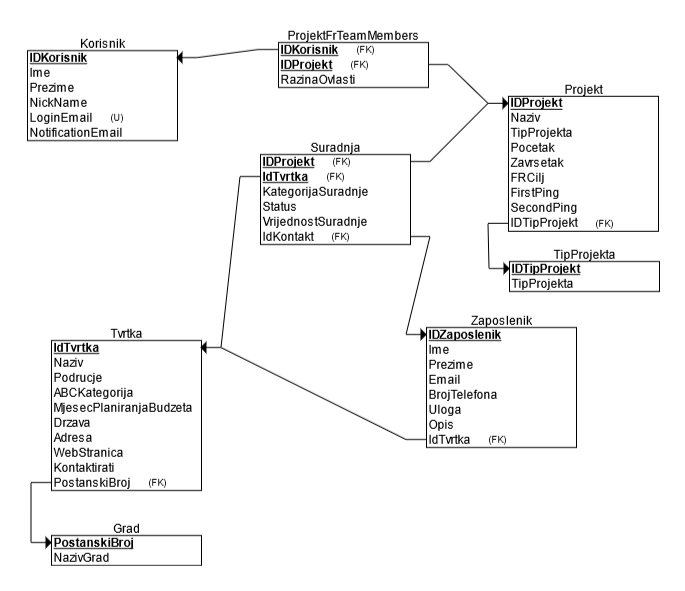
\includegraphics[scale=0.6]{DBDiagram}
					\centering
					\caption{Dijagram baze podataka}
					\label{fig:dbdiagram}
				\end{figure}
				\begin{figure}[H]
					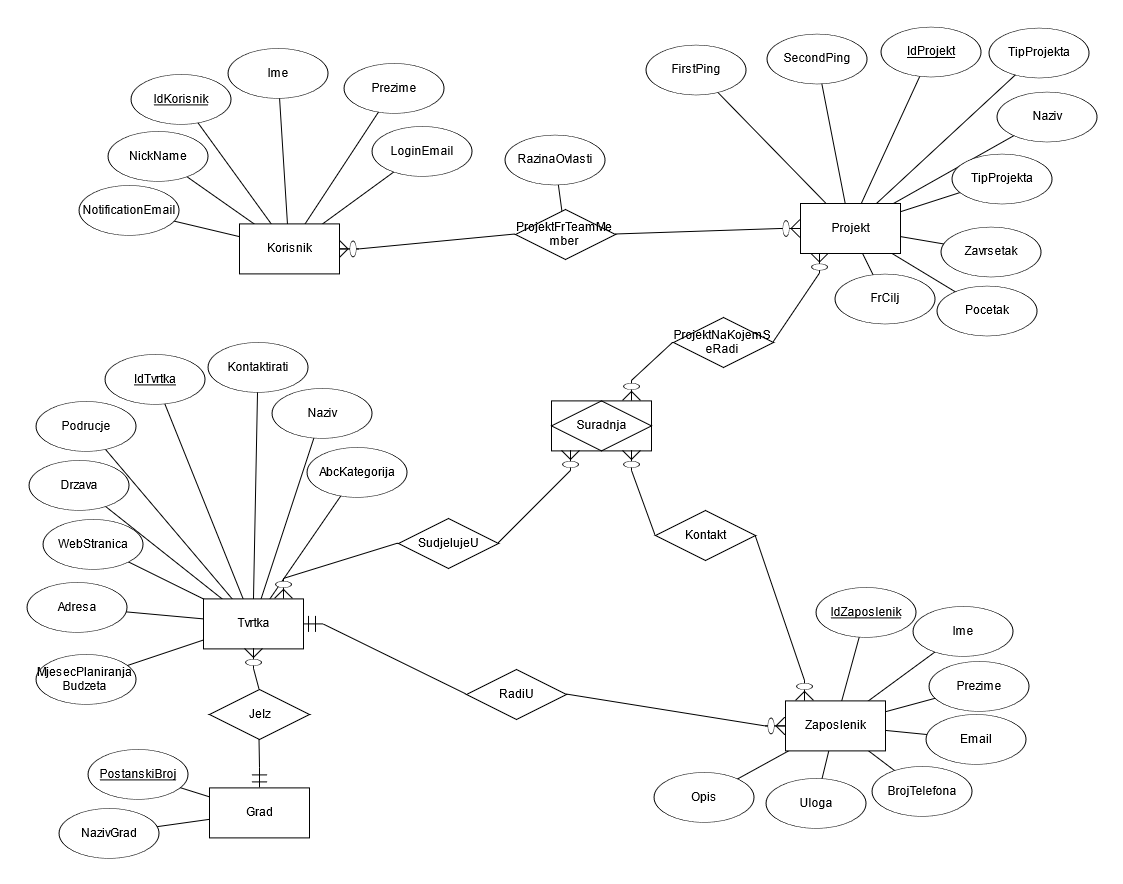
\includegraphics[scale=0.4]{ERDiagram}
					\centering
					\caption{Entity-relationship dijagram}
					\label{fig:erdiagram}
				\end{figure}	
			\eject
			
			
		\section{Dijagram razreda}
		
			Na sljedećim slikama prikazani su UML dijagrami razreda koji se koriste u aplikaciji. Podijeljeni su u 3 dijela. Prvi dijagram prikazuje klase kojima smo modelirali entitete aplikacije, drugi prikazuje DTO-ove \textit{(Data transfer object)}, a treći prikazuje kontrolere. Može se uočiti da postoje veze između klasa iz različitih dijagrama (npr. UserDto sadrži UserSystemAuthority), ali su one izostavljene radi preglednosti.
			
			\begin{figure}[H]
				\includegraphics[scale=0.2]{ModelUML} %veličina slike u odnosu na originalnu datoteku i pozicija slike
				\centering
				\caption{UML dijagram razreda}
				\label{fig:modelUml}
			\end{figure}
			\begin{figure}[H]
				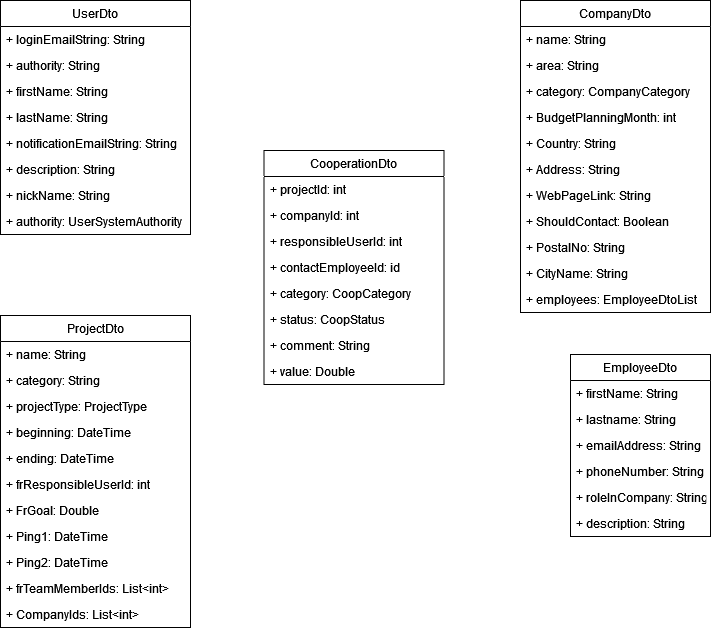
\includegraphics[scale=0.2]{DtoUml} %veličina slike u odnosu na originalnu datoteku i pozicija slike
				\centering
				\caption{UML dijagram Data Transfer Object-a}
				\label{fig:dtouml}
			\end{figure}
			\begin{figure}[H]
				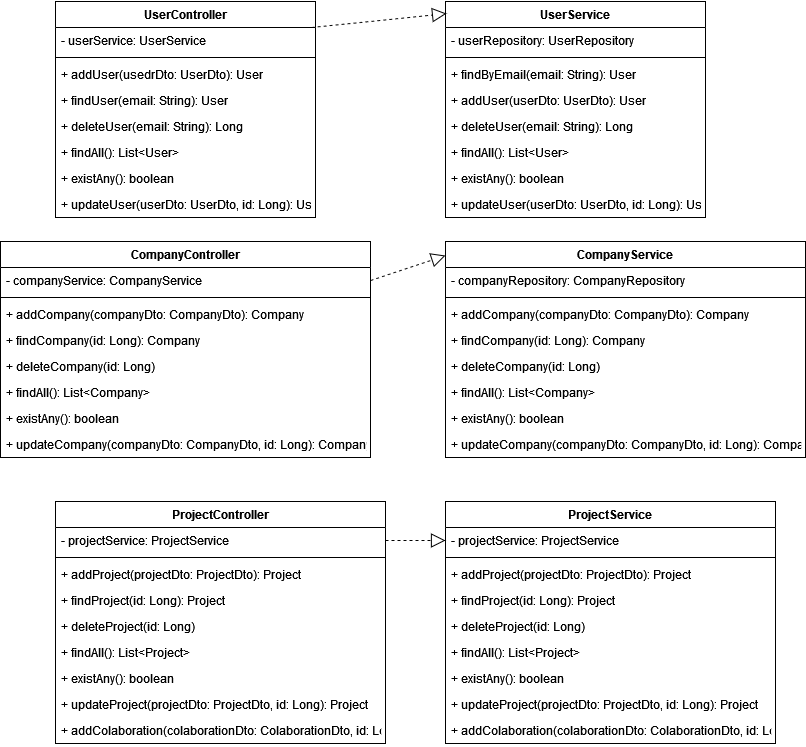
\includegraphics[scale=0.1]{ControllerServiceUml} %veličina slike u odnosu na originalnu datoteku i pozicija slike
				\centering
				\caption{UML dijagram kontrolera i servisa}
				\label{fig:controllersServicesUml}
		\end{figure}
		
	
	\iffalse % block comment (zavrsava sa fi)
	
		\section{Dijagram stanja}
			
			%\textbf{\textit{dio 2. revizije}}\\
			
			%\textit{Potrebno je priložiti dijagram stanja i opisati ga. Dovoljan je jedan dijagram stanja koji prikazuje \textbf{značajan dio funkcionalnosti} sustava. Na primjer, stanja korisničkog sučelja i tijek korištenja neke ključne funkcionalnosti jesu značajan dio sustava, a registracija i prijava nisu. }

			{ Na slici 4.6 prikazan je dijagram stanja oko pravljanja korisnika za administratora.
			Nakon prijave, klijentu se prikazuje početna stranica iz koje dalje prolazi kroz aplikaciju.
			Korisnik na izborniku može odabrati nekoliko mogućnost. Jedna od njih je pregled korinika po kojemu može filtrirati.
			Od tamo može nadoodati korisnika i promijeniti osobne podatke o korisniku. Također može i izbrisati
			korisnika i promijeniti rolu tog korisnika, ako taj korisnik nije zadnji administrator. Administrator s
			početne stranice može i otići na projekte, pa postaviti ili maknuti korisnika sa nekog od projekata}

			\begin{figure}[H]
				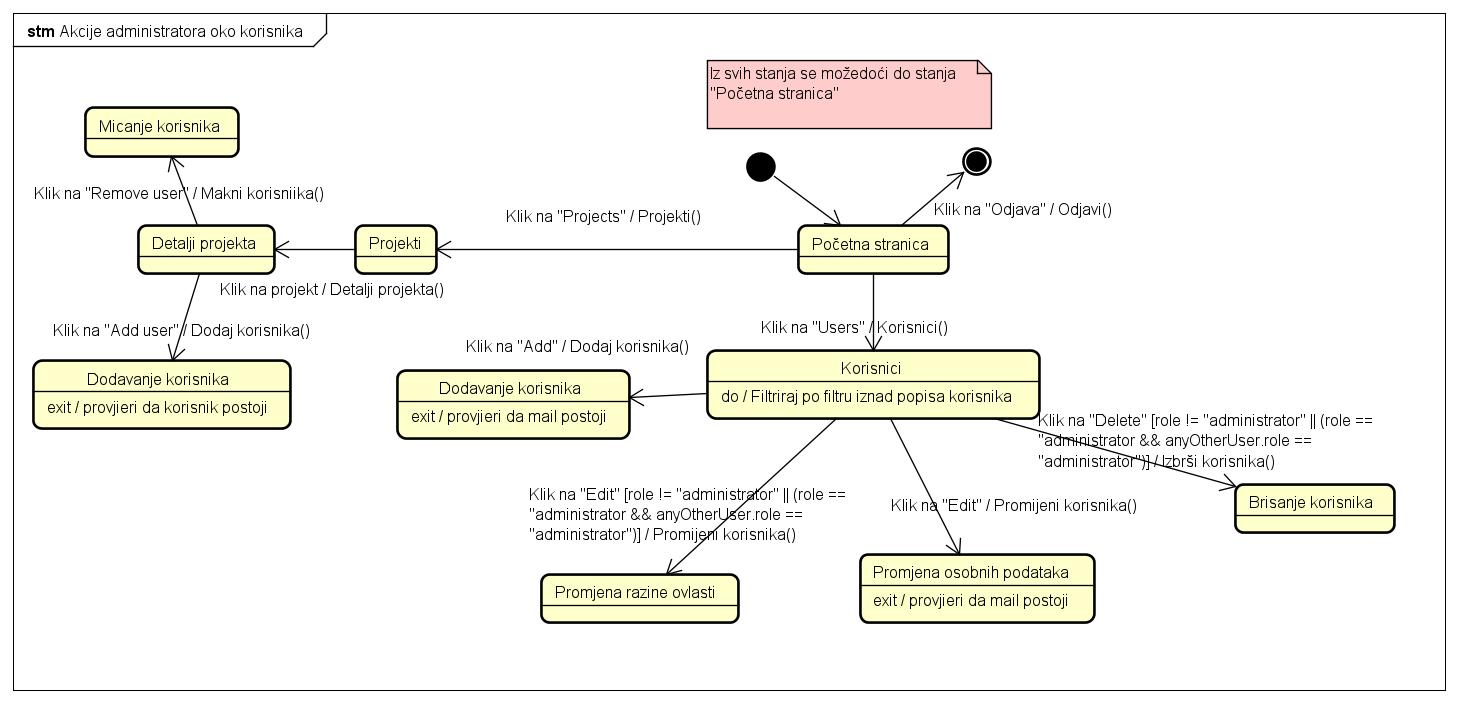
\includegraphics[scale=0.3]{slike/Dijagram stanja}
				\centering
				\caption{Dijagram stanja}
				\label{fig:stanja}
			\end{figure}

			\eject 
		
		\section{Dijagram aktivnosti}
			
			%\textbf{\textit{dio 2. revizije}}\\
			
			 %\textit{Potrebno je priložiti dijagram aktivnosti s pripadajućim opisom. Dijagram aktivnosti treba prikazivati značajan dio sustava.}
			{ Na dijagramu 4.7 prikazan je proces promjene role korisnika. Korisnik se prijavi u sustav,
		  	ode na pregled korisnika i izabere korisnika kojemu želi promijeniti rolu. Tamo može promijeniti sve
			podatke o korisniku, uključujući i rolu. Kada je korisnik zadovoljan promjenama spremi ih.}

			\begin{figure}[H]
				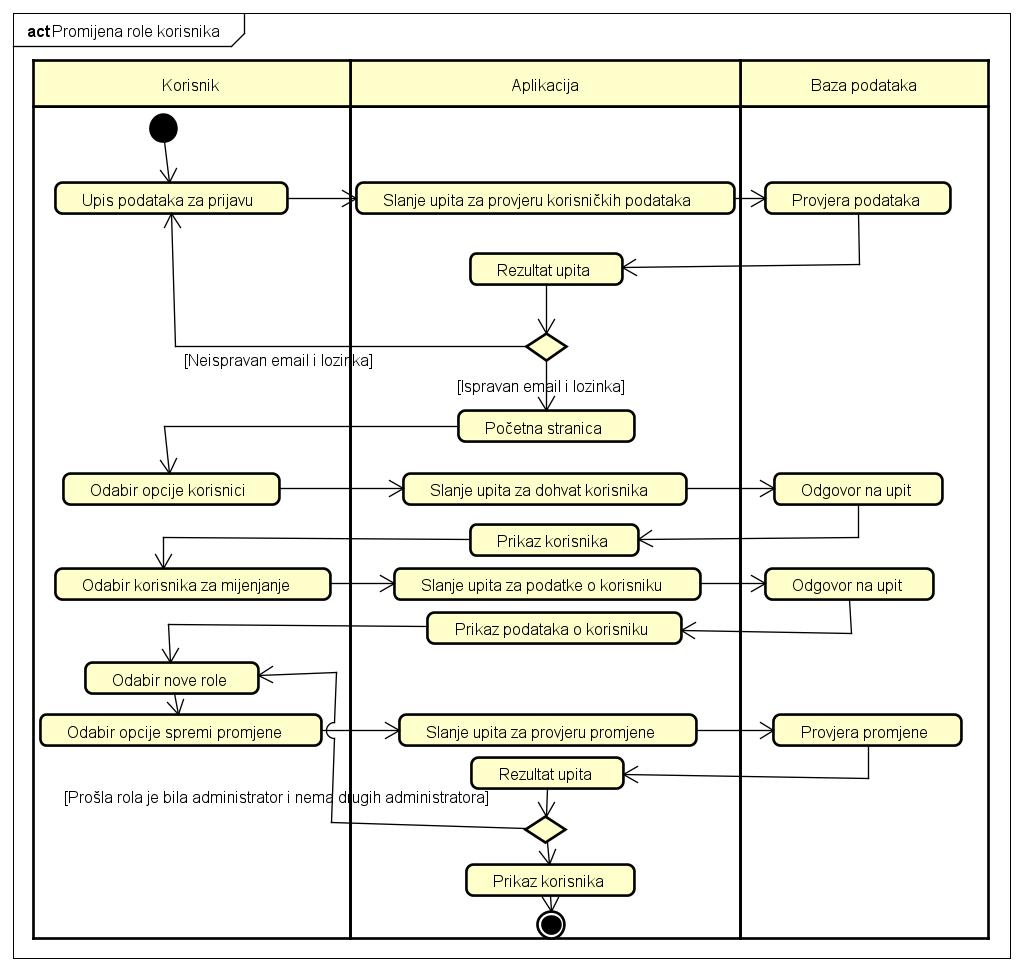
\includegraphics[scale=0.3]{slike/Dijagram aktivnosti}
				\centering
				\caption{Dijagram aktivnosti}
				\label{fig:aktivnosti}
			\end{figure}

			\eject
			
		\section{Dijagram komponenti}
		
			%\textbf{\textit{dio 2. revizije}}\\
		
			 %\textit{Potrebno je priložiti dijagram komponenti s pripadajućim opisom. Dijagram komponenti treba prikazivati strukturu cijele aplikacije.}
			{ Sustavu se pristupa preko dva različita sučelja. Preko sučelja za dohvat HTML, CSS i JS datoteka poslužuju se
			datoteke koje pripadaju frontend dijelu aplikacije. Router je komponenta koja na
			upit s url određuje koja datoteka ce se poslužiti na sučelje. Sve JavaScript datoteke ovise o React biblioteci iz
			koje dohvaćaju gotove komponente kao što su gumbi, forme i slično. Preko sučelja
			za dohvat JSON podataka pristupa se REST API komponenti. REST API posluzuje
			podatke koji pripadaju backend dijelu aplikacije. EntityFrameworkCore je zadužen
			za dohvaćanje tablica iz baze podataka pomoću SQL upita. Podaci koji su pristigli
			iz baze se šalju dalje MVC arhitekturi u obliku DTO. Reactview komponenta preko dostupnih sučelja komunicira sa aplikacijom
			te ovisno o korisnikovim akcijama osvjezava prikaz i dohvača nove podatke ili datoteke }

			\begin{figure}[H]
				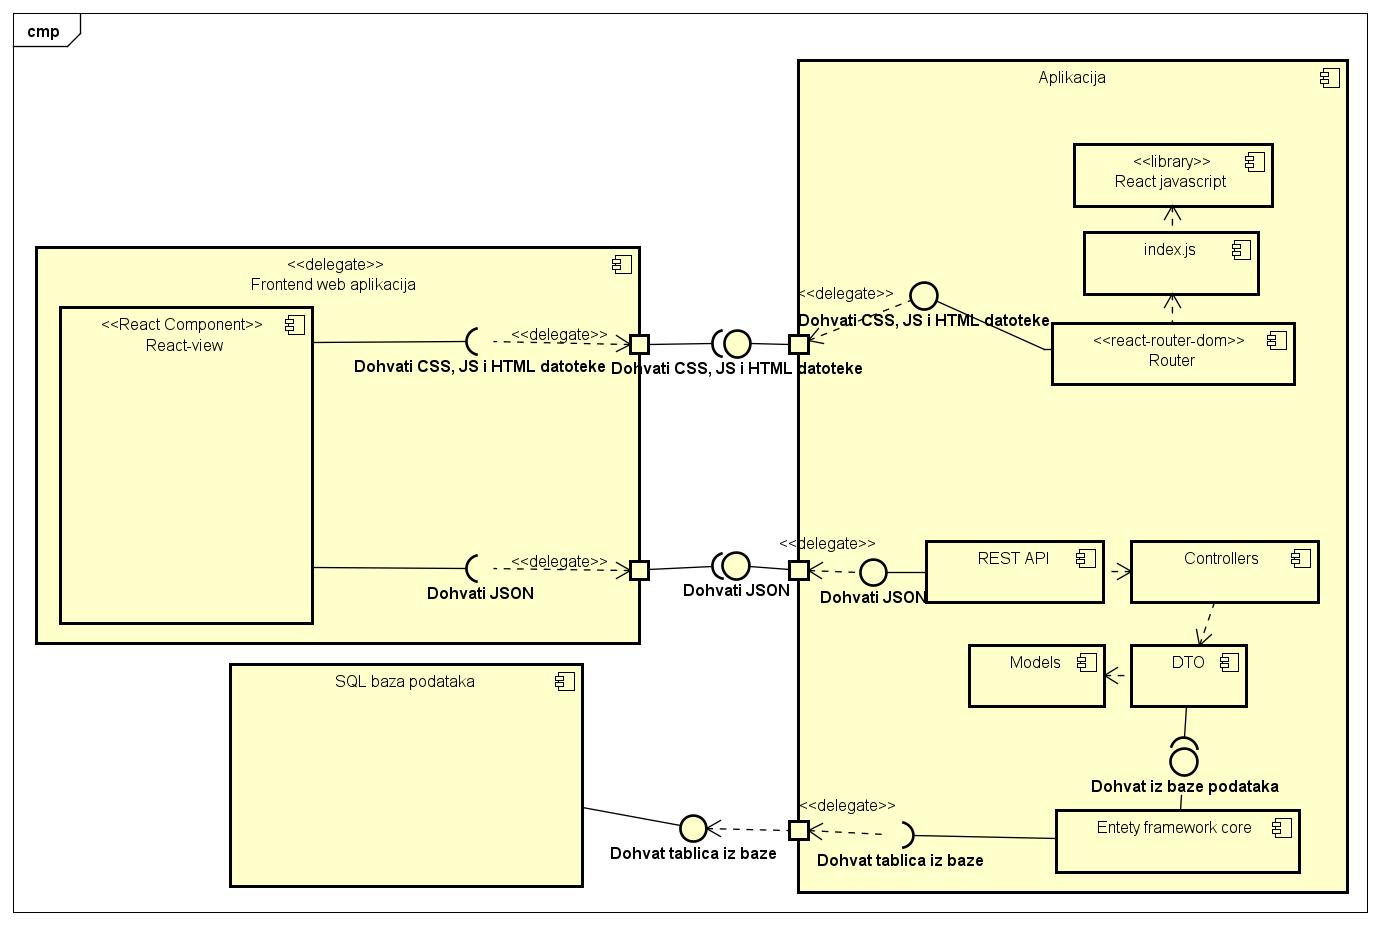
\includegraphics[scale=0.3]{slike/Dijagram komponenti}
				\centering
				\caption{Dijagram komponenti}
				\label{fig:komponente}
			\end{figure}
			 
	\fi % block comment (pocinje sa iffalse)